\section{POSIX Threads Programming}

Für UNIX Systeme steht ein stardardisiertes threads programming interface in C zur Verfügung (POSIX threads / pthreads).


\subsection{UNIX Process vs. UNIX Thread}

\begin{center}
    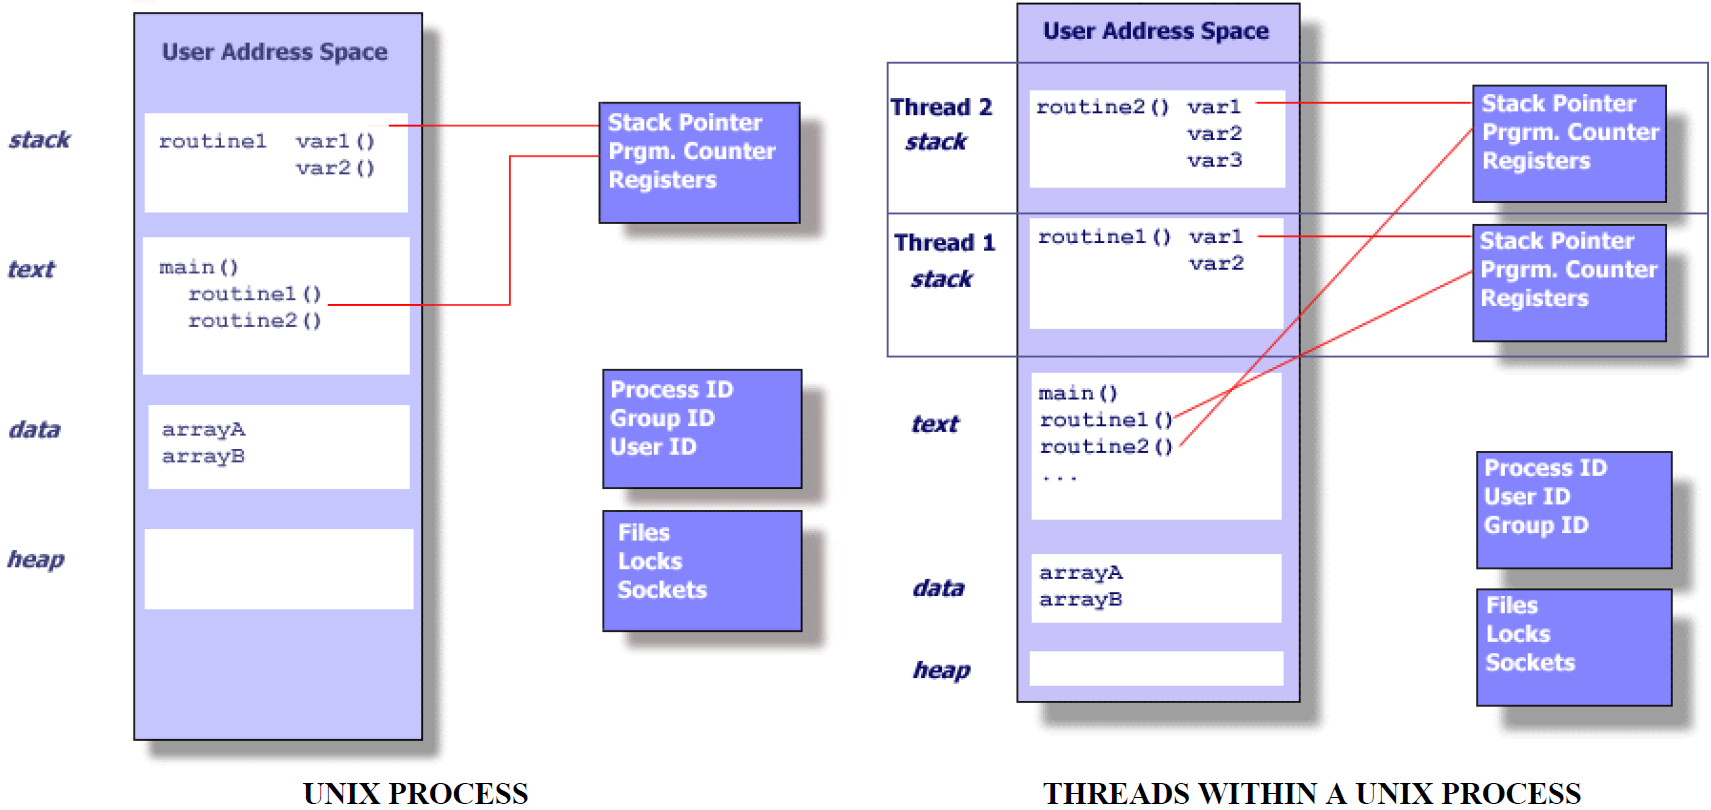
\includegraphics[width=0.75\columnwidth]{images/posix_process_threads.png}
\end{center}


\subsubsection{UNIX Process}

\begin{outline}
    \1 \textbf{heavyweight process} (generiert von Betriebssystem)
    \1 Prozess erfordert \textbf{erheblichen overhead}, da Informationen über Programmressourcen und 
        den Ausführungsstatus des Programms, beispielsweise:
        \2 Prozess-ID, Prozessgruppen-ID, Benutzer-ID und Gruppen-ID
        \2 Environment, Programmanweisungen
        \2 Register, Stack, Heap
        \2 Datei-Deskriptoren, Signal-Aktionen
        \2 Gemeinsame Bibliotheken
        \2 Werkzeuge für die prozessübergreifende Kommunikation
\end{outline}


\subsubsection{UNIX Thread}

\begin{outline}
    \1 lightweight 'process' (weniger overhead)
    \1 Unabhängiger 'stream of instructions', welcher simultan mit anderen 'streams of instructions' ablaufen kann %CHECK: german names...
    \1 Prozedur, welche unabhängig von ihrem (aufrufenden) main-Programm abläuft
    \1 \textbf{Threadsexistieren in einem Prozess und nutzen dessen Ressourcen}
        \2 Sobald ein Prozess ended, enden auch die darin existierenden Threads!
    \1 \textbf{Ein Thread benutzt den gleichen Adressraum wie andere Threads im gleichen Prozess}
        \2 Daten können einfach mit anderen Threads im gleichen Prozess geteilt werden
    \1 Threads werden vom Betriebssystem 'gescheduled'
    \1 Ein Thread dupliziert nur die essenziellen Ressourcen die er braucht, um unabhängig 'schedulable' zu sein:
        \2 Stack pointer, Register
        \2 Scheduling properties (policy / priority)
        \2 Set of pendding and blocked signals  % CHECK: in german...
        \2 Thread-spezifische Daten
\end{outline}

\vspace{0.1cm}

\textbf{ \textrightarrow\ Gleichzeitigkeit wird in der Programmierung mit Threads umgesetzt!}


\subsection{pthreads API}

\subsubsection{Includes / Compile \& Link}

\begin{outline}
    \1 \mylstbox{#include <pthread.h>} wird benötigt
    \1 Methoden der pthreads API starten mit \mylstbox{pthread_}
    \1 Source files, welche pthreads verwenden, sollen mit \mylstbox{-pthread} kompiliert werden
    \1 Für das file-linking muss der command \mylstbox{-lpthread} verwenet werden
\end{outline}


\example{Compiling / Linking file printer.c}

\begin{description}
    \item[Compiling:] \lstinline|clang -c -Wall -pthread printer.c|
    \item[Linking:]   \lstinline|clang -o printer printer.o -Wall -lpthread|
\end{description}


\subsubsection{Thread starten / beenden}

\begin{outline}
    \1 Jede Funktion mit der folgenden interface kann eine Thread-Methode werden
        \2 Als Parameter / Return-Wert sind alle Pointer-Datentypen möglich \\ %CHECK if this is correct...
        \mylstbox[aboveskip=1mm, linewidth=\linewidth, morekeywords={[3], arg}]{void* threadRoutine(void* arg);}
    \1 Ein Thread wird mit der folgenden Funktion gestartet:
        \lstinputlisting[aboveskip=1mm, linewidth=\linewidth, morekeywords={[3], thread, attr, arg}, morekeywords={[2], pthread_t, pthread_attr_t}]{snippets/posix_start_thread.c}
    \1 Ein Thread kann mit einer der folgenden drei Arten beendet werden
        \2 Thread ruft Funktion \mylstbox[aboveskip=1mm]{pthread_exit()} auf
        \2 Thread springt aus Thread Routine \mylstbox[aboveskip=1mm]{startRoutine} zurück
        \2 Thread wird mit Funktion \mylstbox[aboveskip=1mm]{pthread_cancel()} abgebrochen
\end{outline}


\subsubsection{Warten, bis ein Thread beendet ist}

\begin{outline}
    \1 Nach dem Starten des Threads bzw. am Ende des main-Programms kann eine Endlos-Schleife eingefügt werden
        \2 \textbf{Dies sollte nie gemacht werden}, da der Prozess so die gesamten CPU-Ressourcen braucht
    \1 Entsprechende Funktion aus pthreads API verwenden
        \lstinputlisting[aboveskip=1mm, linewidth=\linewidth, morekeywords={[3], thread, attr}, morekeywords={[2], pthread_t, pthread_attr_t}]{snippets/posix_wait_for_thread_termination.c}
\end{outline}


\subsection{Beispiel: thread API}

% \begin{center}
%     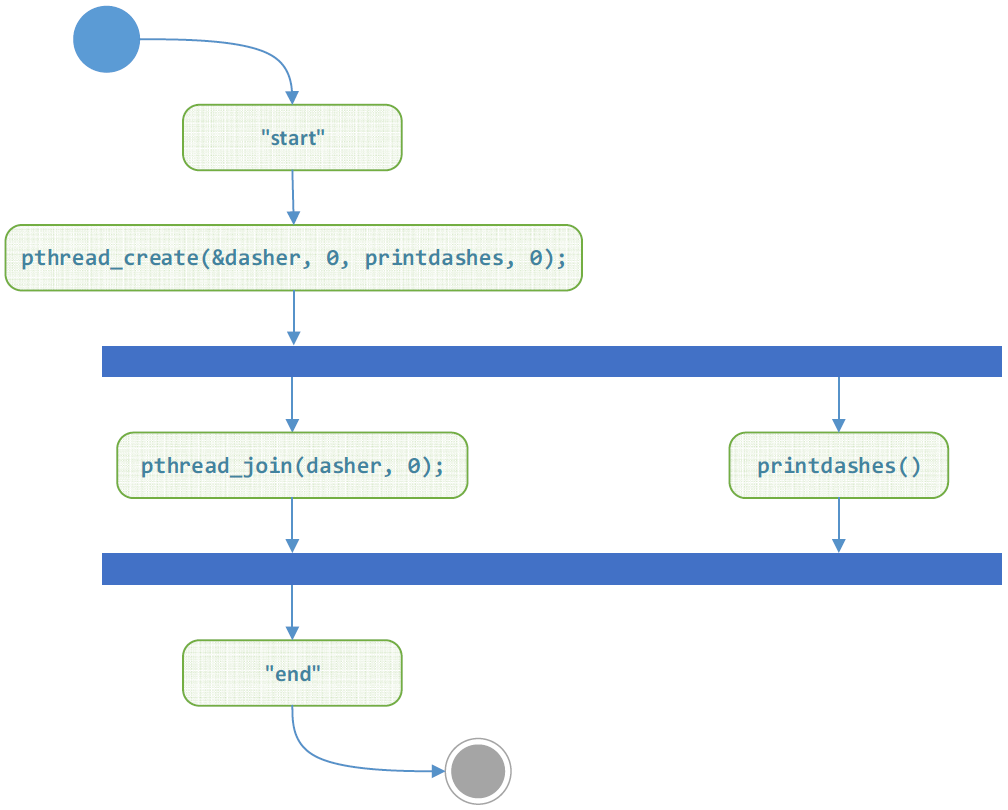
\includegraphics[width=0.8\columnwidth]{images/posix_thread_fork_join.png}
% \end{center}
\begin{minipage}[t]{0.48\columnwidth}
    \lstinputlisting[aboveskip=1mm, firstnumber=1, firstline=1, lastline=23, morekeywords={[3], arg, ret, dasher, i}, morekeywords={[2], pthread_t}]{snippets/posix_join.c}
\end{minipage}
\hfill
\begin{minipage}[t]{0.48\columnwidth}
    \lstinputlisting[aboveskip=1mm, firstnumber=24, firstline=24, lastline=48, morekeywords={[3], arg, ret, dasher, i}, morekeywords={[2], pthread_t}]{snippets/posix_join.c}
\end{minipage}


\subsection{Thread-safeness}
Thread-safeness bezieht sich auf die Fähigkeit einer Anwendung, mehrere Threads gleichzeitig auszuführen,
\textbf{ohne 'clubbering' und 'race conditions'} zu verursachen. Damit Thread-safeness gewährleistet werden kann, ist \textbf{Synchronisation}
erforderlich.

\begin{description}
    \item[clubbering:] Speicher durcheinander bringen, wenn mehrere Threads den gleichen Speicher benötigen und 'falsch' darauf zugreifen
    \item[race conditions:] Programmablauf und Endergebnis hängen davon ab, in welcher Reihenfolge 'gleichzeitig' ablaufende Threads auf z.B. eine
        globale Variable im Speicher zufreifen und das Verhalten somit unvorhersehbar wird
\end{description}


\subsubsection{Empfehlung: Thread-Safeness}

Wenn Thread-safeness nicht explizit garantiert ist (z.B. von einer Library, welche verwendet wird), muss  angenommen werden, dass sie 
\textbf{nicht thread-safe} ist! \\
Um in einem solchen Fall Thread-safeness zu gewährleisten, können die Aufrufe einer 'unsicheren' Funktion \textbf{serialisiert} werden.


\subsection{Quasi-Parallelität / 'Prozess'-Zustände}

\subsubsection{Prozess-Zustände}

\begin{minipage}[t]{0.45\columnwidth}
    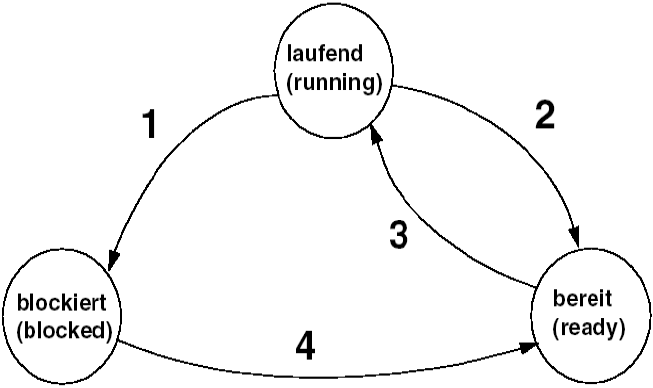
\includegraphics[width=\columnwidth, align=t]{images/posix_process_states.png}
\end{minipage}
\hfill
\begin{minipage}[t]{0.5\columnwidth}
    \begin{enumerate}
        \item I/O Operation, Warten auf Bedingung
        \item Scheduler entzieht CPU
        \item Scheduler weist CPU zu
        \item I/O beendet, Bedigung erfüllt
    \end{enumerate}
\end{minipage}

\vspace{0.2cm}

\begin{minipage}[t]{0.4\columnwidth}
    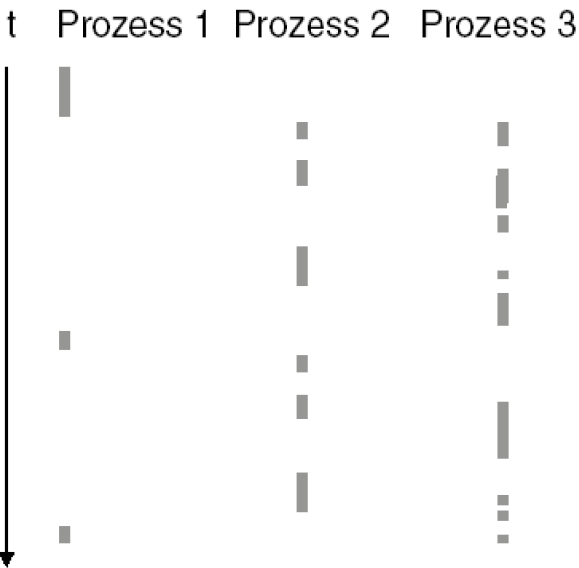
\includegraphics[width=\columnwidth, align=t]{images/concurrency_quasi_parallelitaet.png}
\end{minipage}
\hfill
\begin{minipage}[t]{0.58\columnwidth}
    \raggedright
    \begin{outline}
        \1 Prozesse / Threads warten die 'meiste Zeit' \\
            \textrightarrow\ blocked
        \1 Scheduler ordnet CPU denjenigen Prozess / Thread zu, die im Zustand 'ready' sind und 'etwas zu tun haben'
        \1 Die Zuordnung hängt vom verwendeten Scheduling-Algorithmus ab:
            \2 First come First serve Scheduling: Eine Queue mit allen Prozessen, wobei nächster Prozess jeweils hinten angehängt wird und erster 
                Eintrag der Queue aktuell ausgeführt wird
            \2 Priority Scheduling: Pro Priorität gibt es eine Queue. Abarbeitung je nach Algorithmus anders
    \end{outline}
\end{minipage}

